\documentclass{article}
\usepackage[utf8]{inputenc}
\usepackage{natbib}
\usepackage{graphicx}
\usepackage{comment}
\usepackage{geometry}
\geometry{lmargin = 1 in}
\usepackage[portuges]{babel}

\selectlanguage{portuges}

\title{Decimação}
\author{João Pedro Oliveira Faria}
\date{Abril 2020}

\begin{document}

\begin{titlepage}
\clearpage\maketitle
\thispagestyle{empty}
\end{titlepage}

\tableofcontents

\section{Introdução}

    O principal objetivo deste trabalho consiste na implementação de um módulo no Matlab que permita a diminuição da frequência de amostragem de um sinal por meios digitais, com a finalidade de ocupar menos memória bem como exigir menos cálculos de processamento. Este processo denomina-se downsampling ou decimação.
    Além disso, para que não ocorra o efeito de "aliasing" é necessário aplicar ao sinal previamente amostrado um filtro passa-baixo. O mesmo irá ser desenvolvido usando um filtro elíptico que obedece às seguintes condições:
    
    \raggedright
    \vspace{5mm} %5mm vertical space
    \begin{itemize}
    \item{Ripple na banda passante de 40 dB}
    \item{Ripple na banda de rejeição de 60 dB}
    \item{Largura de banda de transição de 20\% da banda passante.}
    \item{A frequência de amostragem de 8kHz.}
    \end{itemize}
    
\section{Amostragem e Decimação}

    Um sinal em tempo contínuo tem de ser amostrado a uma determinada frequência para poder ser processado digitalmente, isto é, em certos instantes periódicos de tempo, é obtido uma amostra do sinal. Após processamento do mesmo, converte-se o sinal de digital para analógico para ser ouvido, por exemplo.\\ 

\begin{figure}[h!]
\centering
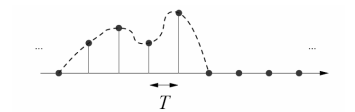
\includegraphics[scale=0.5]{matlab_test_images/outras_imgs/sampling.PNG}
\caption{Amostragem.}
\label{fig:matlab_test_images/outras_imgs/sampling}
\end{figure}
    
    Contudo, mesmo após obtido um sinal amostrado, este pode conter demasiada informação, para o objetivo a que era proposto. Para tal, faz-se um downsampling, isto é, reduz-se o número de amostras do sinal. A decimação pode considerar só uma a cada duas amostras ou uma a cada três amostras, sendo as restantes zero, tratando-se assim de um fator de decimação, N, de dois e três, respetivamente.\\  
    
\begin{figure}[h!]
\centering
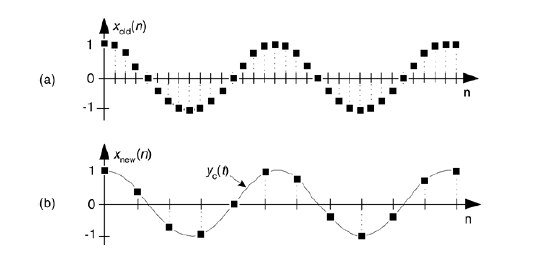
\includegraphics[scale=0.5]{matlab_test_images/outras_imgs/decimation_time.PNG}
\caption{Decimação no tempo discreto.}
\label{fig:matlab_test_images/outras_imgs/decimation_time}
\end{figure}   

\section{Aliasing}

    Ao aplicarmos o processo de redução de amostras descrito anteriormente, podemos provocar "aliasing", caso não seja obedecido o teorema de Nyquist, que indica que a máxima frequência do sinal não deve ser superior a metade da frequência de amostragem. Este efeito faz com que sinais com diferentes frequências sejam indistinguíveis entre si quando amostrados sem obedecer ao teorema acima descrito.\\
    
\begin{figure}[h!]
\centering
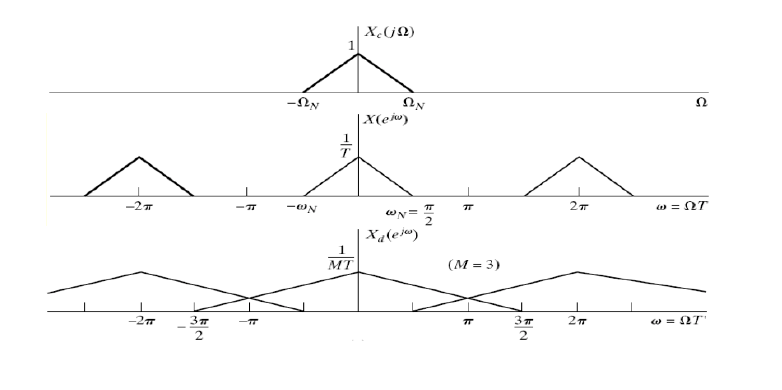
\includegraphics[scale=0.5]{matlab_test_images/outras_imgs/decimacao_aliasing.PNG}
\caption{Decimação com aliasing, fator de decimação M=3.}
\label{fig:matlab_test_images/outras_imgs/decimacao_aliasing}
\end{figure}      
    

    
    Consequentemente, em vez de alterarmos a frequência de amostragem podemos aplicar um filtro passa-baixo para eliminarmos o efeito. Contudo, o mesmo é inexequível dado a sua natureza não causal, daí surgirem várias alternativas, cada uma com vantagens e desvantagens, que se aproximam do filtro ideal. Neste projeto, será implementado o filtro elíptico, cujo nome deriva do facto de os seus pólos no plano s formarem uma elipse.\\
    
\begin{figure}[h!]
\centering
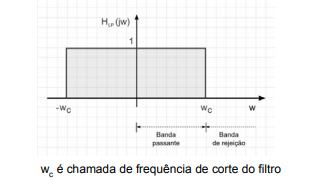
\includegraphics[scale=0.5]{matlab_test_images/outras_imgs/ideal_fil.PNG}
\caption{Filtro ideal passa-baixo.}
\label{fig:matlab_test_images/outras_imgs/ideal_fil}
\end{figure}    
    
\newpage
\section{Filtro elíptico}
  
    
    A resposta em frequência apresenta "ripples" tanto na banda passante como na de rejeição, como a combinação dos filtros chebysheb tipo 1 e 2, apresentando um roll-off mais acentuado que ambos.   

\begin{figure}[h!]
\centering
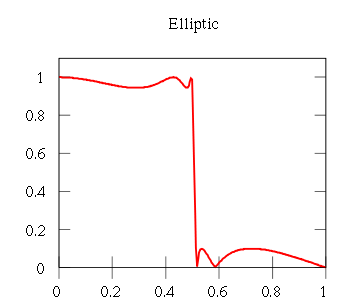
\includegraphics[scale=0.6]{matlab_test_images/outras_imgs/Ellip.png}
\caption{Filtro elíptico resposta em frequência (amplitude).}
\label{fig:matlab_test_images/outras_imgs/Ellip}
\end{figure}    
    
    
\raggedright
\vspace{5mm} %5mm vertical space
\begin{itemize}
\item{O declive da banda de transição é  N*20dB por Década.}
\item{A fase pouco se assemelha a uma reta.}
\item{É uma generalização dos filtros Butterworth e Chebyshev.}
\item{Possui zeros além de pólos.}
\item{Possui um par(es) de zeros imaginários perto da frequência corte que aumenta o declive banda transição.}
\end{itemize}
   
\raggedright
\vspace{5mm} %5mm vertical space
    
\begin{figure}
\begin{center}

\ $
{\displaystyle G_{n}(\omega)={1 \over {\sqrt {1+\epsilon ^{2}R_{n}^{2}(\xi ,\omega /\omega _{0})}}}}$
\caption{Resposta em frequência do filtro elíptico.}

\end{center}
\end{figure}
    
\raggedright
\vspace{5mm} %5mm vertical space
 
Os vários parâmetros que se encontram na equação da figura 6 designam-se:

\begin{itemize}
\item{$\epsilon$ fator de ripple, influencia a amplitude dos "ripples" em ambas as bandas passante e rejeição. \\}
\item{$R_n$, ordem nth da função racional elítica, que define a o gráfico do filtro, recorrendo aos seguintes parâmetros: \\}
\item{$\xi$, fator seletividade, afeta o ripple na banda de rejeição.\\}
\item{$\omega_o$, a frequência de corte, havendo na sua vizinhança um acentuado declive de ganho.  \\}
\end{itemize}

\section{Código Matlab}    
\newpage
\begin{figure}[h]
\begin{center}
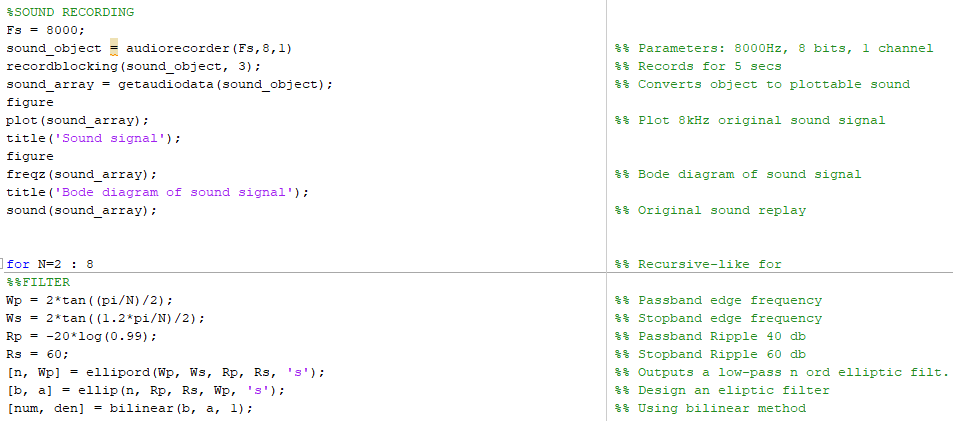
\includegraphics[width=19cm]{matlab_test_images/code_imgs/c1.PNG}
\end{center}
\end{figure}
\newpage
\begin{figure}[h]
\begin{center}
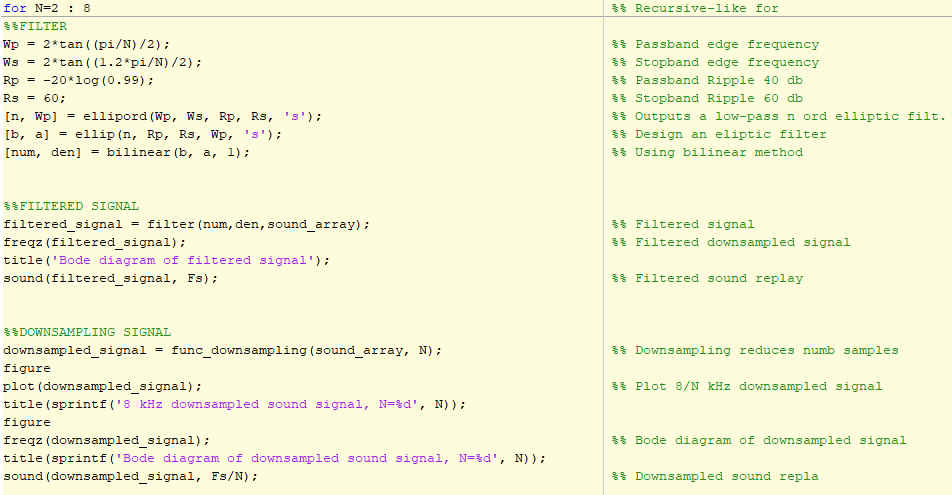
\includegraphics[width=19cm]{matlab_test_images/code_imgs/c2.png}
\end{center}
\end{figure}
\newpage
\begin{figure}[h]
\begin{center}
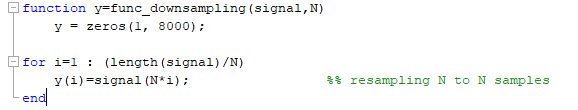
\includegraphics[width=19cm]{matlab_test_images/code_imgs/c3.png}
\end{center}
\end{figure}
\newpage
\begin{figure}[h]
\begin{center}
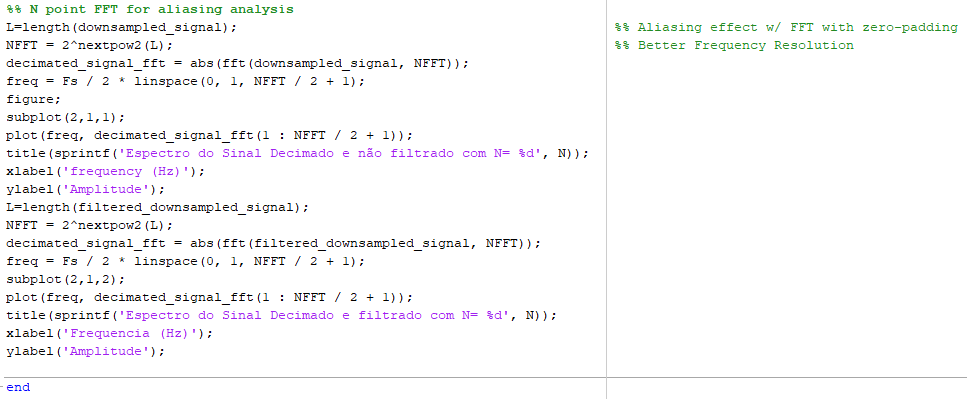
\includegraphics[width=19cm]{matlab_test_images/code_imgs/c4.png}
\end{center}
\end{figure}
\newpage
\begin{figure}[h]
\begin{center}
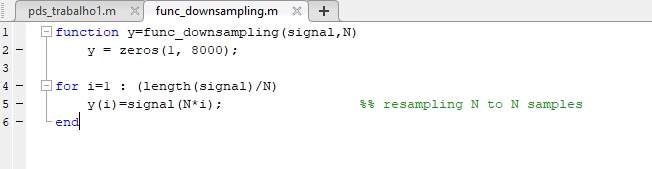
\includegraphics[width=19cm]{matlab_test_images/code_imgs/c5.png}
\end{center}
\end{figure}
\newpage

\section{Testes e Resultados}    

Os excertos de som foram amostrados recorrendo ao uso das seguintes funções de Matlab:
\raggedright
\vspace{5mm} %5mm vertical space

    -audiorecord, que foi implementada para captar o som à frequência proposta de 8kHZ, 8bits, definida em 1 canal, gerando um objeto de som; \\
    -recordblocking, que apenas grava durante 3 segundos, neste teste, o som; \\
    -getaudiodata, que converte o objeto som num array de doubles para poder ser manipulável, por outras funções Matlab, o sinal captado; \\
    
    Quanto ao resto das funções, existe documentação na forma de comentários associada ao código.
    
    Foi utilizada a música "Afraid to Shoot Strangers" dos Iron Maiden dado que possui a voz do cantor, bem
    como uma guitarra e bateria para diversificar o espetro de frequências do sinal entrada.

    Após discretização do sinal, o mesmo foi filtrado, decimado, por diferentes fatores de decimação (N), variando de 2 a 8, e decimado/amostrado bem como foi ainda efetuado um teste de aliasing (análise FFT de n-pontos) para mostrar como o filtro passa-baixo usado elimina este efeito para todos os N.
    Por último, foi analisado os diagramas de bode dos diferentes filtros gerados, via método bilinear, para diferentes N, e o seu efeito final no som, que foi convertido para contínuo para comparar não só visualmente, mas auditivamente o mesmo ao fim de cada uma das etapas, sendo estas reportadas de seguida no relatório.
    
   
\begin{figure}[h!]
\centering
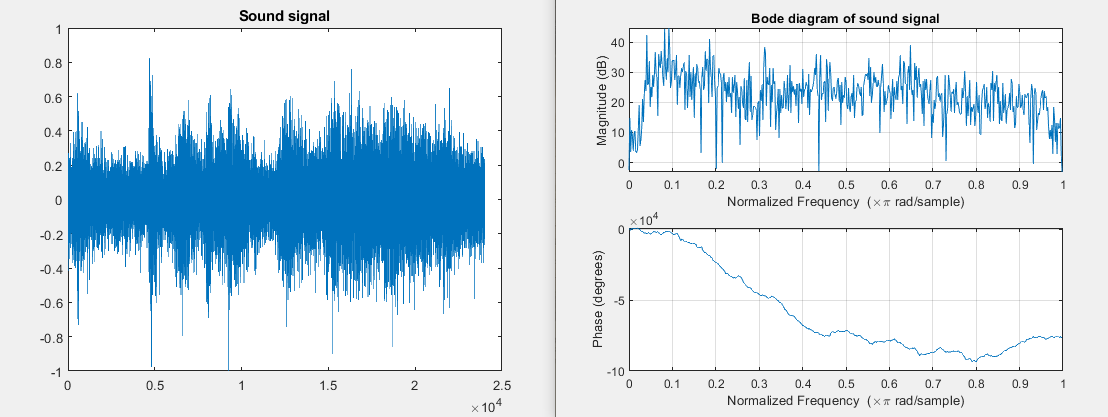
\includegraphics[scale=0.5]{matlab_test_images/som_org.PNG}
\caption{Som original a 8 kHz e o seu diagrama de bode, à direita.}
\label{fig:matlab_test_images/som_org}
\end{figure}  
\newpage


\subsection{N = 2}
\vfill
\begin{figure}[h!]
\centering
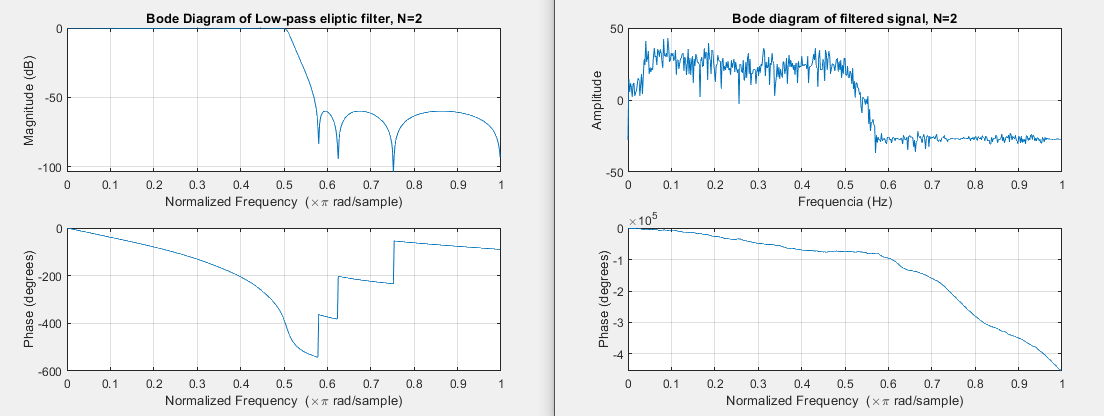
\includegraphics[scale=0.5]{matlab_test_images/cut_images/fil2.PNG}
\caption{Diagrama bode (DB) do filtro, à esquerda, e do sinal filtrado, à direita.}
\label{fig:matlab_test_images/cut_images/fil2}
\end{figure}
\begin{figure}[h!]
\centering
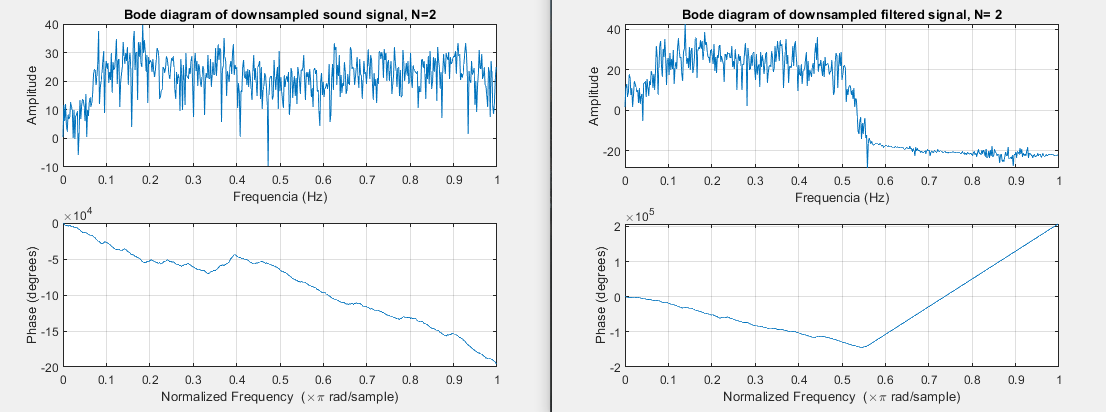
\includegraphics[scale=0.5]{matlab_test_images/cut_images/fil3.PNG}
\caption{DB do sinal decimado, à esquerda, e do sinal filtrado e decimado, à direita.}
\label{fig:matlab_test_images/cut_images/fil3}
\end{figure}  
\newpage
\begin{figure}[h!]
\centering
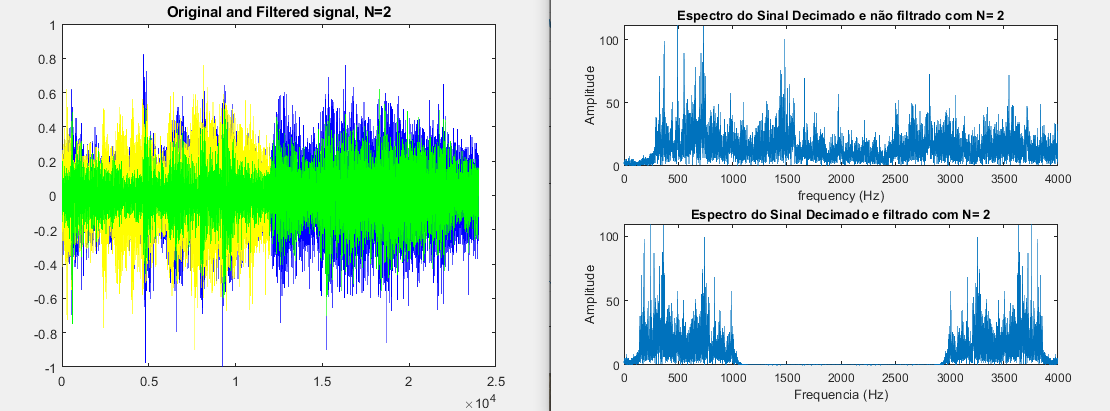
\includegraphics[scale=0.5]{matlab_test_images/cut_images/fil4.PNG}
\caption{Na esquerda, o sinal original (azul) com o sinal decimado, sem zeros (amarelo) e sinal filtrado e subamostrado (verde). Na direita, a FFT dos sinais decimado, com aliasing (cima) e decimado e filtrado (baixo), sem aliasing.}
\label{fig:matlab_test_images/cut_images/fil4}
\end{figure}  

\raggedright
\vspace{5mm} %5mm vertical space

Para N=2, tanto para o sinal filtrado como para o sinal não filtrado se assemelham ao sinal original, sendo estes mais graves um bocado que o inicialmente captado. Voz, guitarra, bateria são facilmente distinguíveis.
Contudo, no  sinal não filtrado, nota-se uma leve distorção na voz e na guitarra.

\newpage


\subsection{N = 3}
\vfill
\begin{figure}[h!]
\centering
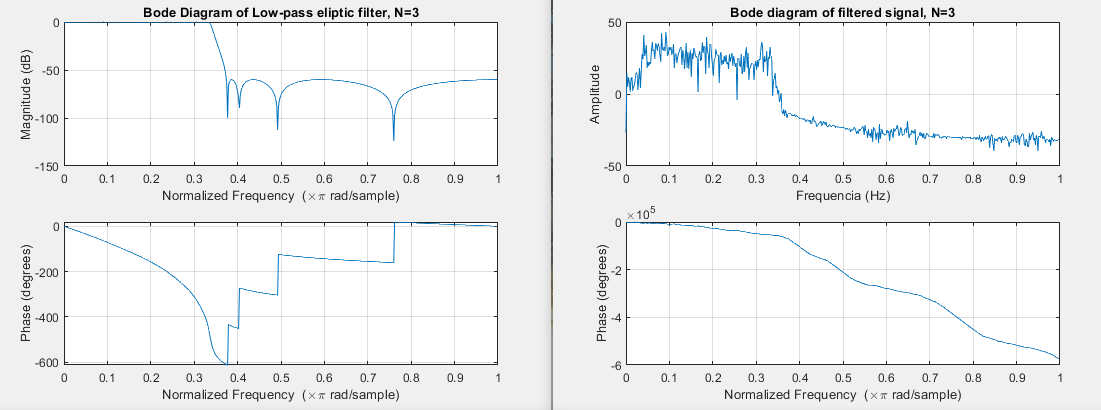
\includegraphics[scale=0.5]{matlab_test_images/cut_images/fil5.PNG}
\caption{Diagrama bode (DB) do filtro, à esquerda, e do sinal filtrado, à direita.}
\label{fig:matlab_test_images/cut_images/fil5}
\end{figure}
\begin{figure}[h!]
\centering
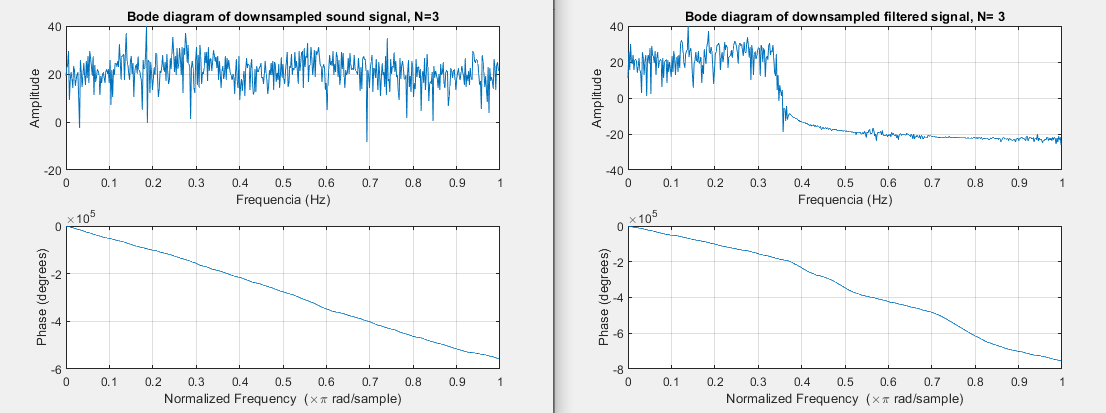
\includegraphics[scale=0.5]{matlab_test_images/cut_images/fil6.PNG}
\caption{DB do sinal decimado, à esquerda, e do sinal filtrado e decimado, à direita.}
\label{fig:matlab_test_images/cut_images/fil6}
\end{figure}  
\newpage
\begin{figure}[h!]
\centering
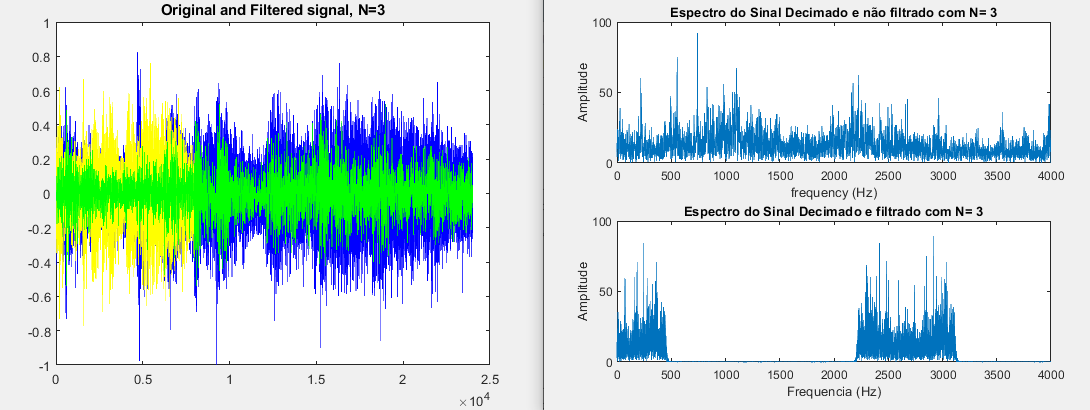
\includegraphics[scale=0.5]{matlab_test_images/cut_images/fil7.PNG}
\caption{Na esquerda, o sinal original (azul) com o sinal decimado, sem zeros (amarelo) e sinal filtrado e subamostrado (verde). Na direita, a FFT dos sinais decimado, com aliasing (cima) e decimado e filtrado (baixo), sem aliasing.}
\label{fig:matlab_test_images/cut_images/fil7}
\end{figure}  

\raggedright
\vspace{5mm} %5mm vertical space

Para N=3, ambos os sinais são mais graves, contudo, agora é o som filtrado o menos percetível, sendo o mais grave. Com algum esforço ainda se consegue ouvir sons que representam a voz e a guitarra para o filtrado; quanto ao não filtrado ainda se ouve, com dificuldade, os três diferentes timbres com alguma clareza.
Ouve-se, ainda que um pouco baixo, um barulho fundo.

\newpage

\subsection{N = 4}
\vfill
\begin{figure}[h!]
\centering
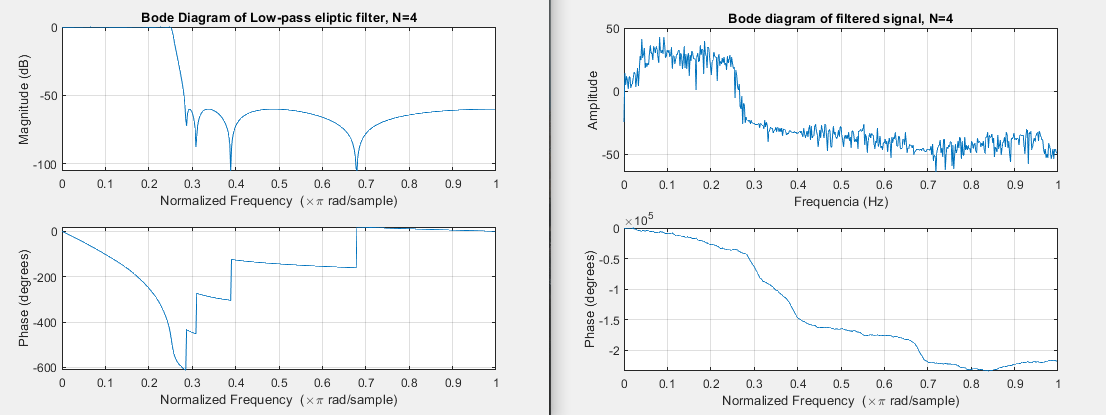
\includegraphics[scale=0.5]{matlab_test_images/cut_images/fil8.PNG}
\caption{Diagrama bode (DB) do filtro, à esquerda, e do sinal filtrado, à direita.}
\label{fig:matlab_test_images/cut_images/fil8}
\end{figure}
\begin{figure}[h!]
\centering
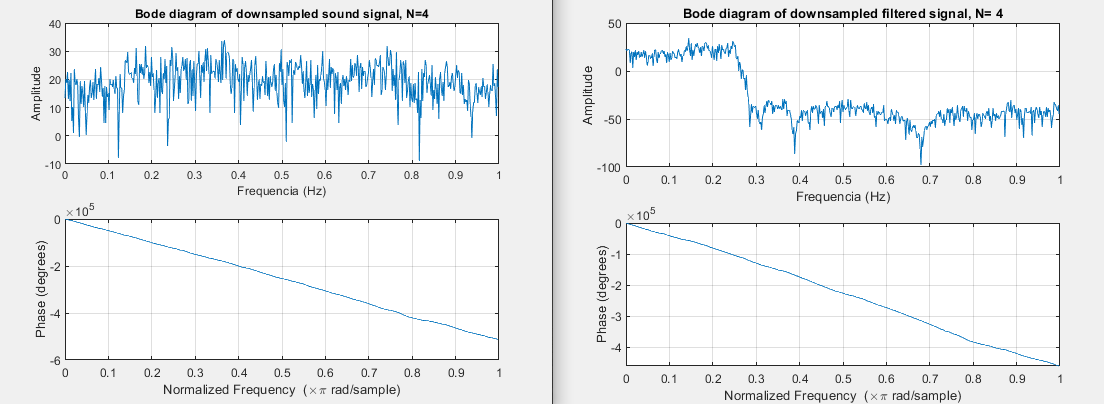
\includegraphics[scale=0.5]{matlab_test_images/cut_images/fil9.PNG}
\caption{DB do sinal decimado, à esquerda, e do sinal filtrado e decimado, à direita.}
\label{fig:matlab_test_images/cut_images/fil9}
\end{figure}  
\newpage
\begin{figure}[h!]
\centering
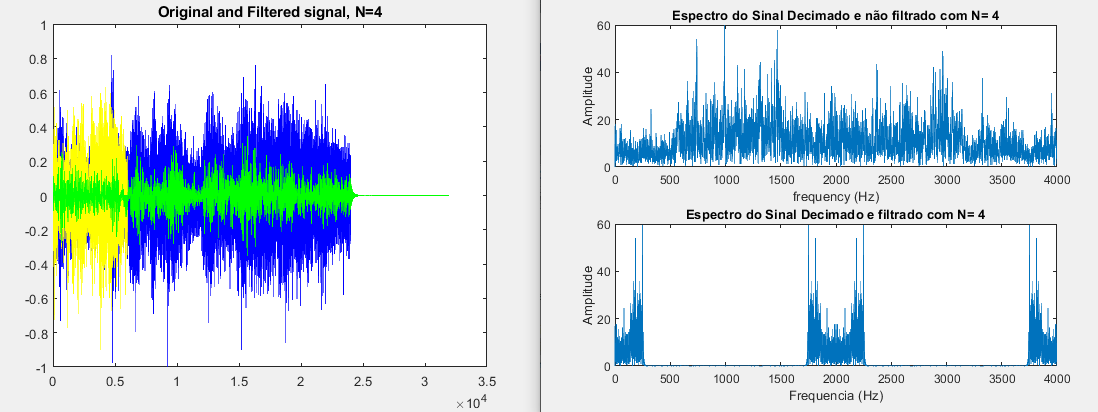
\includegraphics[scale=0.5]{matlab_test_images/cut_images/fil10.PNG}
\caption{Na esquerda, o sinal original (azul) com o sinal decimado, sem zeros (amarelo) e sinal filtrado e subamostrado (verde). Na direita, a FFT dos sinais decimado, com aliasing (cima) e decimado e filtrado (baixo), sem aliasing.}
\label{fig:matlab_test_images/cut_images/fil10}
\end{figure}  

\raggedright
\vspace{5mm} %5mm vertical space

Para N=4, do som não filtrado ouve-se sons que se podem assemelhar aos timbres mencionados(voz, guitarra, bateria).
Do som filtrado, só os batuques dados na bateria é que são minimamente percetíveis.
Sinais mais graves, ouve-se um barulho fundo geral.

\newpage

\subsection{N = 5}
\vfill
\begin{figure}[h!]
\centering
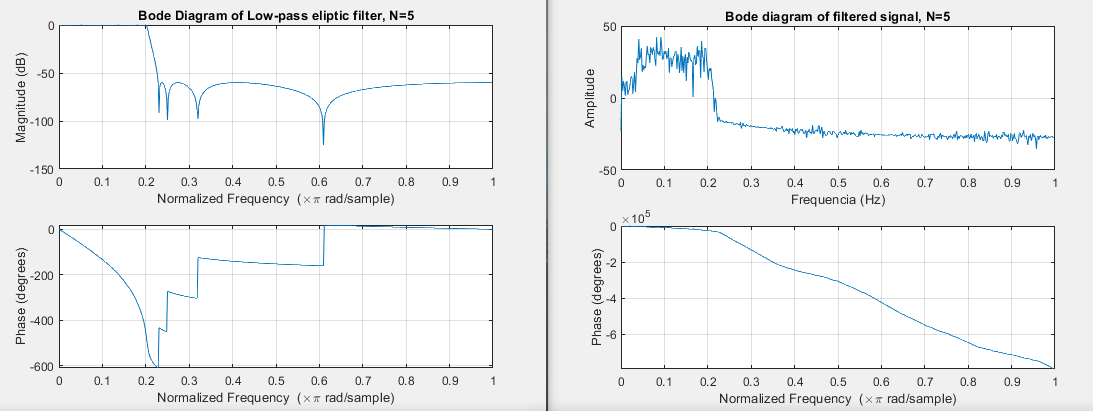
\includegraphics[scale=0.5]{matlab_test_images/cut_images/fil11.PNG}
\caption{Diagrama bode (DB) do filtro, à esquerda, e do sinal filtrado, à direita.}
\label{fig:matlab_test_images/cut_images/fil11}
\end{figure}
\begin{figure}[h!]
\centering
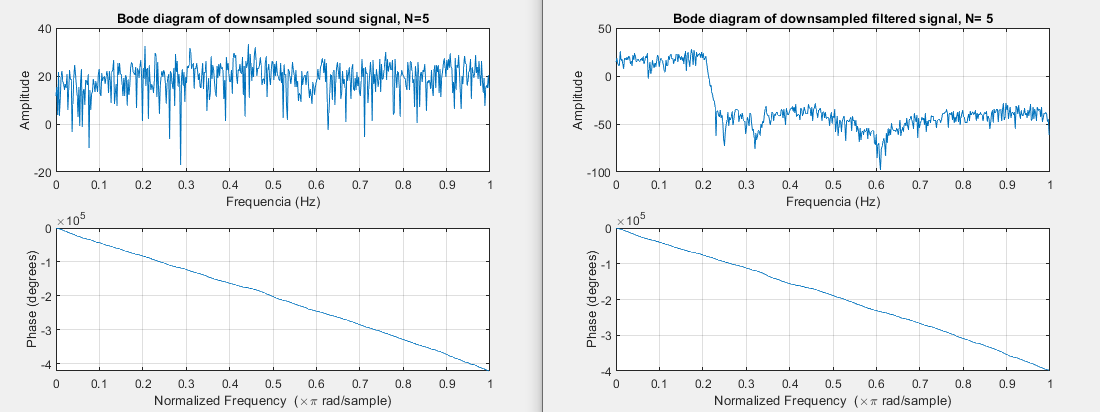
\includegraphics[scale=0.5]{matlab_test_images/cut_images/fil12.PNG}
\caption{DB do sinal decimado, à esquerda, e do sinal filtrado e decimado, à direita.}
\label{fig:matlab_test_images/cut_images/fil12}
\end{figure}  
\newpage
\begin{figure}[h!]
\centering
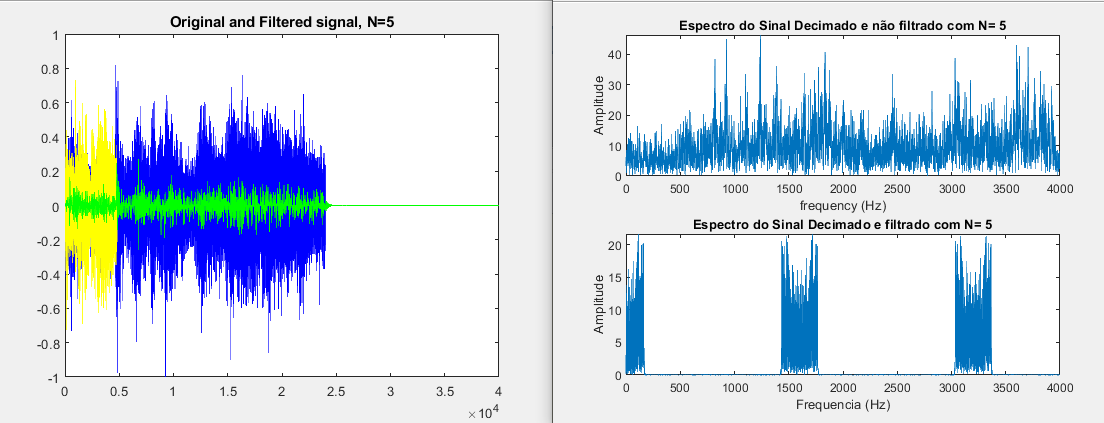
\includegraphics[scale=0.5]{matlab_test_images/cut_images/fil13.PNG}
\caption{Na esquerda, o sinal original (azul) com o sinal decimado, sem zeros (amarelo) e sinal filtrado e subamostrado (verde). Na direita, a FFT dos sinais decimado, com aliasing (cima) e decimado e filtrado (baixo), sem aliasing.}
\label{fig:matlab_test_images/cut_images/fil13}
\end{figure}  

\raggedright
\vspace{5mm} %5mm vertical space

Para N=5, o som não filtrado encontra-se ainda mais distorcido, já não se percebe a guitarra e a letra é difícil de perceber.
O outro não é mais que um barulho de fundo.

\newpage

\subsection{N = 6}
\vfill
\begin{figure}[h!]
\centering
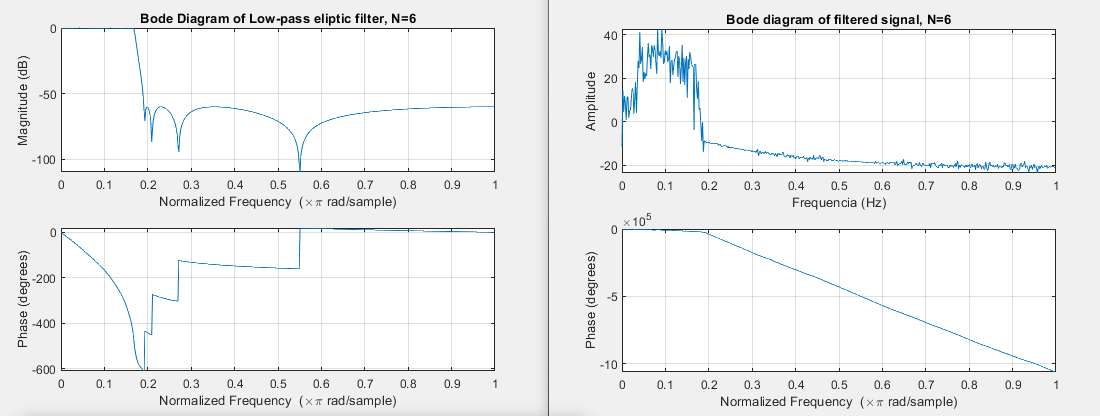
\includegraphics[scale=0.5]{matlab_test_images/cut_images/fil14.PNG}
\caption{Diagrama bode (DB) do filtro, à esquerda, e do sinal filtrado, à direita.}
\label{fig:matlab_test_images/cut_images/fil14}
\end{figure}
\begin{figure}[h!]
\centering
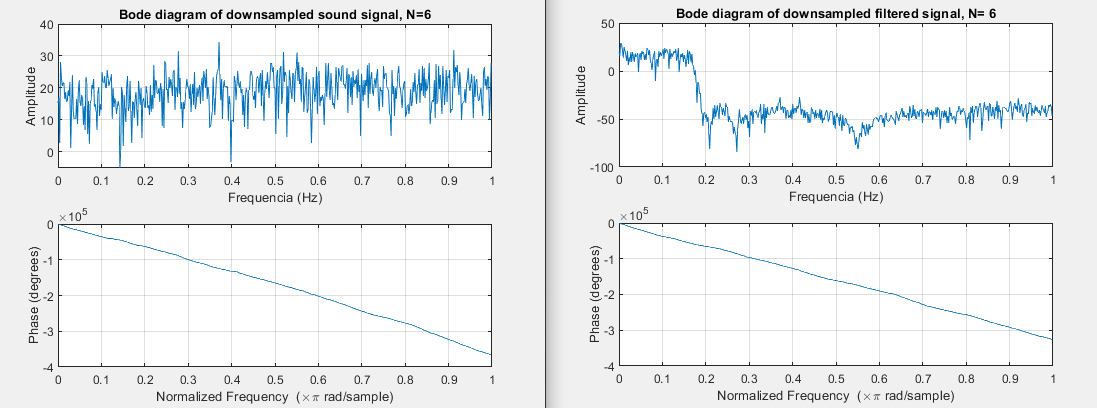
\includegraphics[scale=0.5]{matlab_test_images/cut_images/fil15.PNG}
\caption{DB do sinal decimado, à esquerda, e do sinal filtrado e decimado, à direita.}
\label{fig:matlab_test_images/cut_images/fil15}
\end{figure}  
\newpage
\begin{figure}[h!]
\centering
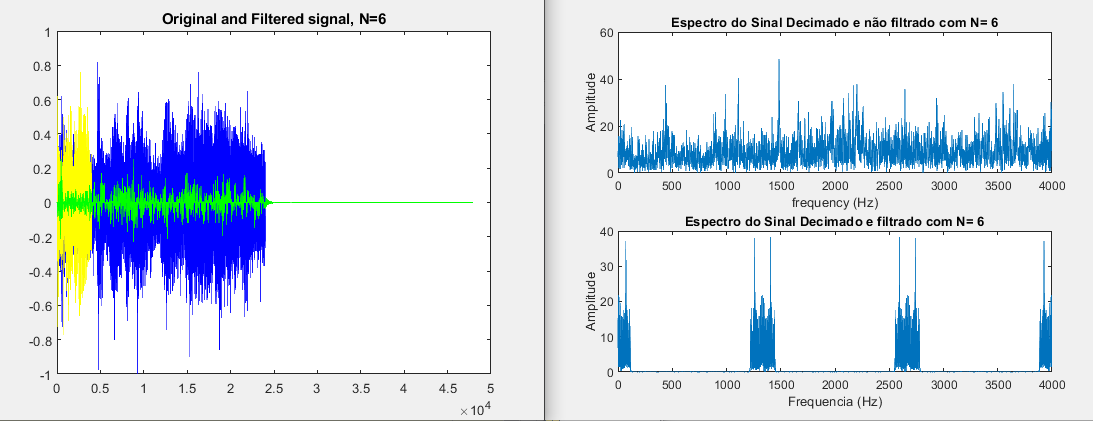
\includegraphics[scale=0.5]{matlab_test_images/cut_images/fil16.PNG}
\caption{Na esquerda, o sinal original (azul) com o sinal decimado, sem zeros (amarelo) e sinal filtrado e subamostrado (verde). Na direita, a FFT dos sinais decimado, com aliasing (cima) e decimado e filtrado (baixo), sem aliasing.}
\label{fig:matlab_test_images/cut_images/fil16}
\end{figure}  

\raggedright
\vspace{5mm} %5mm vertical space

Para N=6, apenas a voz permanece, sendo muito difícil perceber a letra.
Em ambos os sinais, ouve-se um barulho vindo das profundezas, maioritariamente para o pré-filtrado.
Mal se ouve a bateria.

\newpage

\subsection{N = 7}
\vfill
\begin{figure}[h!]
\centering
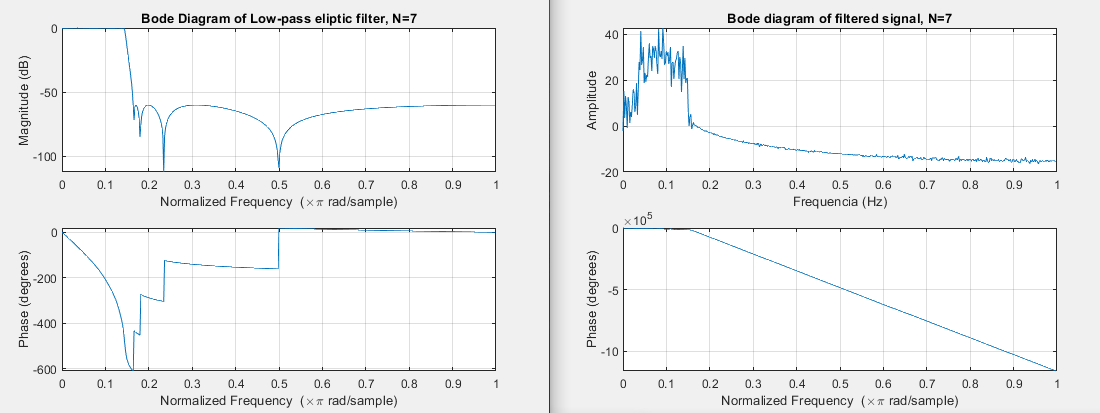
\includegraphics[scale=0.5]{matlab_test_images/cut_images/fil17.PNG}
\caption{Diagrama bode (DB) do filtro, à esquerda, e do sinal filtrado, à direita.}
\label{fig:matlab_test_images/cut_images/fil17}
\end{figure}
\begin{figure}[h!]
\centering
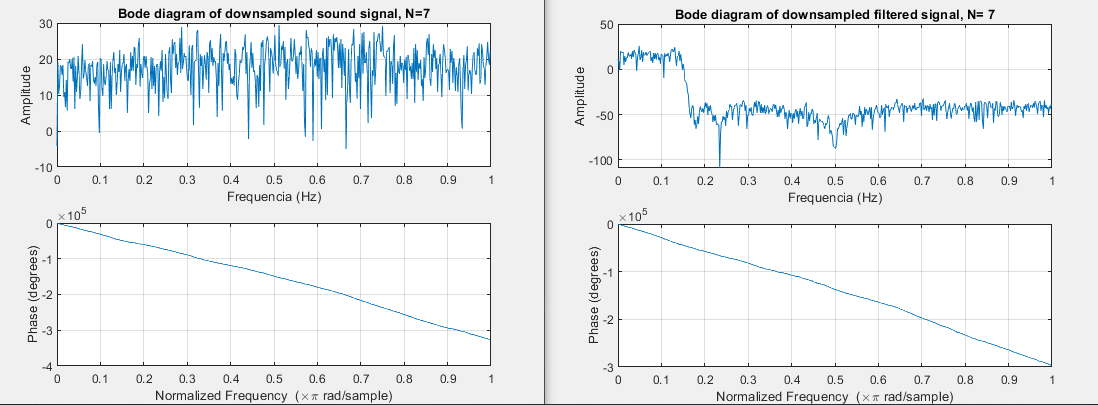
\includegraphics[scale=0.5]{matlab_test_images/cut_images/fil18.PNG}
\caption{DB do sinal decimado, à esquerda, e do sinal filtrado e decimado, à direita.}
\label{fig:matlab_test_images/cut_images/fil18}
\end{figure}  
\newpage
\begin{figure}[h!]
\centering
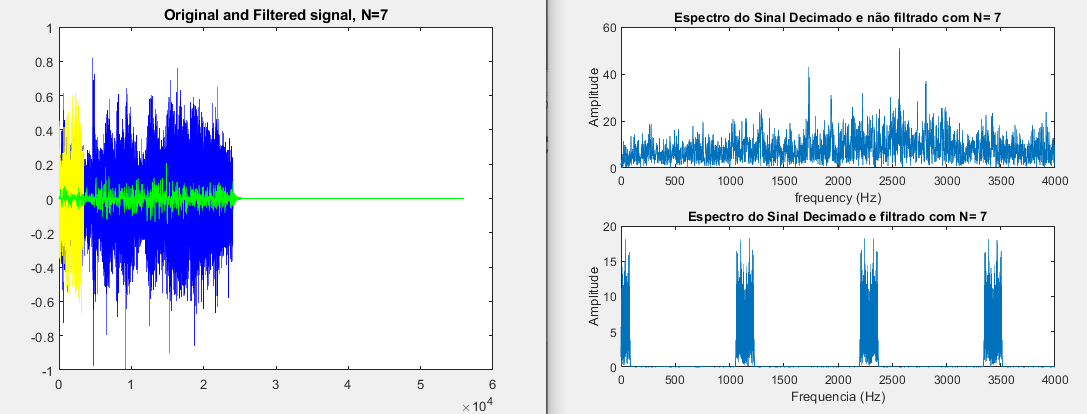
\includegraphics[scale=0.5]{matlab_test_images/cut_images/fil19.PNG}
\caption{Na esquerda, o sinal original (azul) com o sinal decimado, sem zeros (amarelo) e sinal filtrado e subamostrado (verde). Na direita, a FFT dos sinais decimado, com aliasing (cima) e decimado e filtrado (baixo), sem aliasing.}
\label{fig:matlab_test_images/cut_images/fil19}
\end{figure}  

\raggedright
\vspace{5mm} %5mm vertical space

Para N=7, muito mal se percebe a voz do som não filtrado. Continua um barulho de fundo no outro sinal.
Não se ouve bateria.

\newpage

\subsection{N = 8}
\vfill
\begin{figure}[h!]
\centering
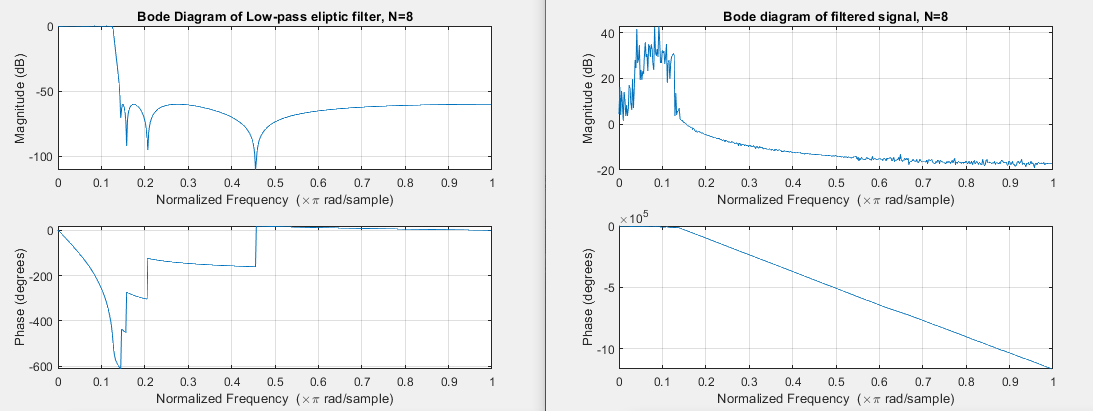
\includegraphics[scale=0.5]{matlab_test_images/cut_images/fil20.PNG}
\caption{Diagrama bode (DB) do filtro, à esquerda, e do sinal filtrado, à direita.}
\label{fig:matlab_test_images/cut_images/fil20}
\end{figure}
\begin{figure}[h!]
\centering
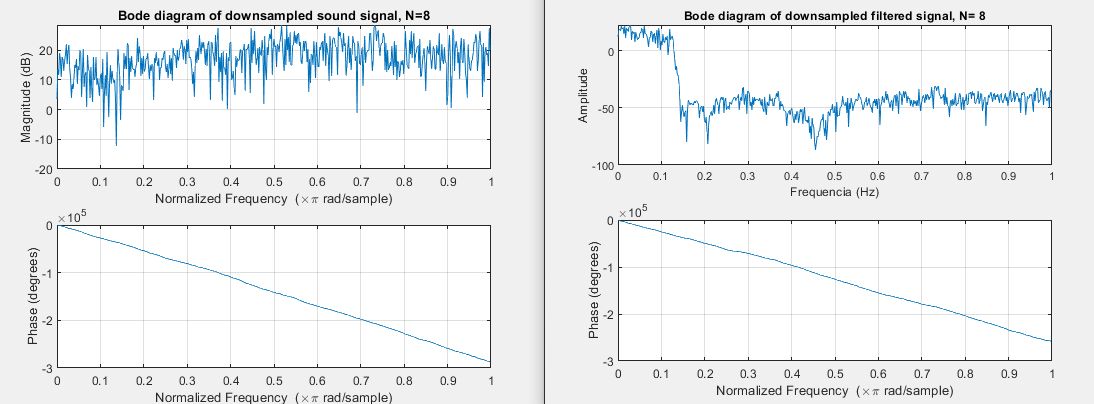
\includegraphics[scale=0.5]{matlab_test_images/cut_images/fil21.PNG}
\caption{DB do sinal decimado, à esquerda, e do sinal filtrado e decimado, à direita.}
\label{fig:matlab_test_images/cut_images/fil21}
\end{figure}  
\newpage
\begin{figure}[h!]
\centering
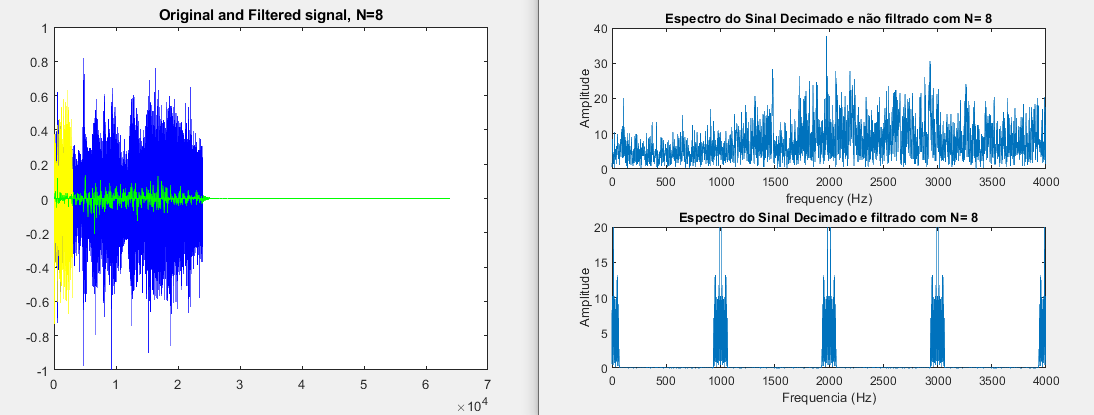
\includegraphics[scale=0.5]{matlab_test_images/cut_images/fil22.PNG}
\caption{Na esquerda, o sinal original (azul) com o sinal decimado, sem zeros (amarelo) e sinal filtrado e subamostrado (verde). Na direita, a FFT dos sinais decimado, com aliasing (cima) e decimado e filtrado (baixo), sem aliasing.}
\label{fig:matlab_test_images/cut_images/fil22}
\end{figure}  

\raggedright
\vspace{5mm} %5mm vertical space

Para N=8, ambos os sinais nada se assemelham à música. Sendo o filtrado, mais grave.

\newpage

\section{Conclusão}    
Analisados os resultados, pode-se verificar que o filtro elíptico, ao filtrar frequências muito elevadas, ajuda a evitar o fenómeno do aliasing (menos distorção do sinal, menos ruído) conforme verificado nas últimas duas imagens de cada subsecção dedicada a cada N, contudo, como visto no diagrama de bode deste, e do sinal filtrado, a banda passante tende a encurtar com o aumento de N, levando à perda de cada vez mais informação.\\
Nota-se que os filtros elípticos são os que apresentam maior roll-off em detrimento das outras versões de filtro, permitindo um corte mais eficiente das amostras, embora, apresentam mais "ripple", mais instabilidade, mais variações de ganho em ambas as bandas de transição e de rejeição.\\
Em suma, existe um balanço a ser efetuado de forma a escolher um filtro que permita a compactação do sinal, para ser mais facilmente processado e ocupar menos memória sem, no entanto, perder demasiada informação relevante. Cabe ao projetista pensar nisso e desenvolver filtros, que não têm de ser elípticos, e ajustá-los da maneira mais conveniente à sua aplicação.\\

\section{Github} 

O projeto irá ser colocado num repositório online para acesso do código, ficheiros latex, imagens, entre outros ficheiros.
\newline
\href{https://github.com/Joaovsky/PDS}

\end{document}
